% This file was created with tikzplotlib v0.10.1.
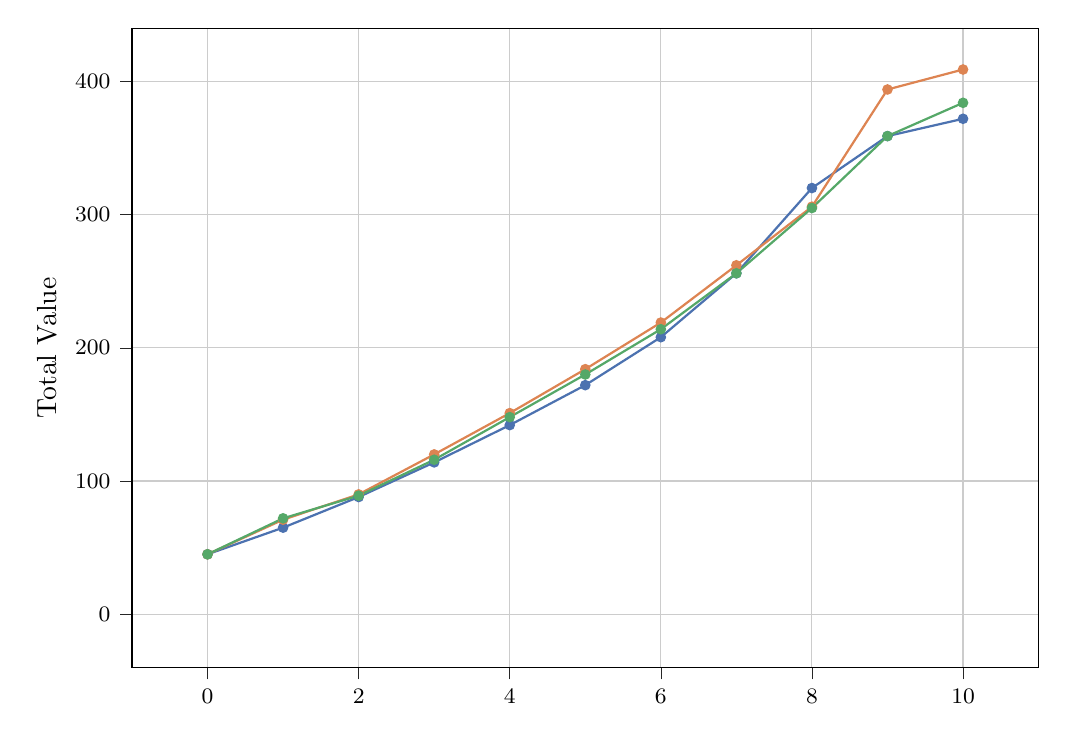
\begin{tikzpicture}

\definecolor{darkslategrey38}{RGB}{38,38,38}
\definecolor{lightgrey204}{RGB}{204,204,204}
\definecolor{mediumseagreen85168104}{RGB}{85,168,104}
\definecolor{peru22113282}{RGB}{221,132,82}
\definecolor{steelblue76114176}{RGB}{76,114,176}

% \begin{axis}[
% axis line style={lightgrey204},
% legend cell align={left},
% legend style={
%   fill opacity=0.8,
%   draw opacity=1,
%   text opacity=1,
%   at={(0.03,0.97)},
%   anchor=north west,
%   draw=lightgrey204
% },
% tick align=outside,
% title={Resource Value Trend},
% x grid style={lightgrey204},
% xmajorgrids,
% xmajorticks=false,
% xmin=-0.5, xmax=10.5,
% xtick style={color=darkslategrey38},
% y grid style={lightgrey204},
% ylabel=\textcolor{darkslategrey38}{Total Value},
% ymajorgrids,
% ymajorticks=false,
% ymin=26.8, ymax=427.2,
% ytick style={color=darkslategrey38}
% ]
\begin{axis}[
legend cell align={left},
legend style={
  fill opacity=0.8,
  draw opacity=1,
  text opacity=1,
  at={(0.03,0.97)},
  anchor=north west,
  draw=lightgrey204,
  font=\footnotesize
},
width=1.08\textwidth,    % 设置宽度
    height=0.8\textwidth,  % 16:9比例
    axis line style={black},
    legend style={fill opacity=0.9, draw opacity=1, text opacity=1, draw=lightgrey204},
    tick align=outside,     % 刻度线向外
    xtick={0,2,4,6,8,10},
    % xticklabels={Initial,Flourishing,Endgame},
    xticklabel style={font=\footnotesize},
    y grid style={lightgrey204},
    ylabel=Total Value,
   ylabel style={font=\footnotesize,
            inner sep=0pt,    % 减少标签和轴的距离
            yshift=-8pt       % 微调标签位置
        },
    ymajorgrids,
    ytick={0,100,200,300,400},
    yticklabel style={font=\footnotesize},
    ymin=0, ymax=400,
    xtick style={color=darkslategrey38},
    ytick style={color=darkslategrey38},
    enlarge x limits=0.1,
    enlarge y limits=0.1,
    grid=major,
    grid style={lightgrey204},
    tick style={color=darkslategrey38},
    axis lines=box,        % 保持完整边框
    x axis line style={black},
    y axis line style={black},
    % 控制刻度线的显示
    tick pos=left,         % y轴刻度线只在左侧显示
    xtick pos=bottom,      % x轴刻度线只在底部显示
    clip=true              % 裁剪超出的内容
]

\addplot [thick, steelblue76114176, mark=*, mark size=1.5, mark options={solid}]
table {%
0 45
1 65
2 88
3 114
4 142
5 172
6 208
7 256
8 320
9 359
10 372
};
% \addlegendentry{Alice}
\addplot [thick, peru22113282, mark=*, mark size=1.5, mark options={solid}]
table {%
0 45
1 71
2 90
3 120
4 151
5 184
6 219
7 262
8 306
9 394
10 409
};
% \addlegendentry{Bob}
\addplot [thick, mediumseagreen85168104, mark=*, mark size=1.5, mark options={solid}]
table {%
0 45
1 72
2 89
3 116
4 148
5 180
6 214
7 256
8 305
9 359
10 384
};
% \addlegendentry{Carol}
\end{axis}

\end{tikzpicture}
